% interactapasample.tex
% v1.05 - August 2017

\documentclass[]{interact}

\usepackage{epstopdf}% To incorporate .eps illustrations using PDFLaTeX, etc.
\usepackage[caption=false]{subfig}% Support for small, `sub' figures and tables
%\usepackage[nolists,tablesfirst]{endfloat}% To `separate' figures https://it.overleaf.com/project/5bbc5c481ace70551dd2c703and tables from text if required
%\usepackahttps://it.overleaf.com/project/5bbc5c481ace70551dd2c703ge[doublespacing]{setspace}% To produce a `double spaced' document if required
%\setlength\parindent{24pt}% To increase paragraph indentation when line spacing is doubled
\usepackage{soul}
\usepackage{amsmath,amssymb} 
\usepackage[natbibapa,nodoi]{apacite}% Citation support using apacite.sty. Commands using natbib.sty MUST be deactivated first!
\setlength\bibhang{12pt}% To set the indentation in the list of references using apacite.sty. Commands using natbib.sty MUST be deactivated first!
\renewcommand\bibliographytypesize{\fontsize{10}{12}\selectfont}% To set the list of references in 10 point font using apacite.sty. Commands using natbib.sty MUST be deactivated first!
\theoremstyle{plain}% Theorem-like structures provided by amsthm.sty
\newtheorem{theorem}{Theorem}[section]
\newtheorem{lemma}[theorem]{Lemma}
\newtheorem{corollary}[theorem]{Corollary}
\newtheorem{proposition}[theorem]{Proposition}

\theoremstyle{definition}
\newtheorem{definition}[theorem]{Definition}
\newtheorem{example}[theorem]{Example}

\theoremstyle{remark}
\newtheorem{remark}{Remark}
\newtheorem{notation}{Notation}

\usepackage[pdftex,colorlinks=true,urlcolor=blue,citecolor=black,anchorcolor=black,linkcolor=black]{hyperref}
\usepackage{xcolor}
\newcommand{\mengyi}[1]{\textcolor{blue}{#1}}
\newcommand{\erica}[1]{\textcolor{red}{#1}}

\usepackage{algorithm} 
\usepackage{algorithmic} 
\renewcommand{\algorithmicrequire}{ \textbf{Input:}} %Use Input in the format of Algorithm
\usepackage{soul}
\usepackage{todonotes}

\begin{document}

%\articletype{ARTICLE TEMPLATE}% Specify the article type or omit as appropriate

\title{Mathematical Programming Representation of Discrete-Event Simulation}
\maketitle
\begin{abstract}

\end{abstract}

\section{Introduction}
Discrete Event Simulation (DES) is one of the most used tool for performance evaluation of %discrete event dynamic
complex systems and, hence, simulation--optimization algorithms are widely used %developed for optimizing the parameters of such systems. 
when performance evaluation has to be coupled with optimization, i.e., when the best system configuration, according to some criteria, has to be found meanwhile guaranteeing a given value of some performance measure.  
Most of the state--of--the--art simulation--optimization algorithms consider DES as a black--box function, and the structure of DES has been seldom studied. Under the black--box setting, simulation--optimization algorithms works in an iterative way, alternating simulation and optimization procedures, and always require %huge amount of 
many iterations to explore the %search 
feasible region of the optimization problem, %and can be
thus possibly leading to %computationally inefficient. 
computational inefficiency.
On the contrary, a minority of the simulation--optimization literature explores the structure of the DES, and %that
such research is referred to as white--box simulation--optimization. The benefit of white--box simulation--optimization is the saving of simulation budget due to the fact that %since 
the optimization procedure is guided by the information contained in the structure of DES. However, the barrier to the use of white--box simulation--optimization is how to model DES as white--box, so that it eventually favors the optimization. In this work, %we present 
how to establish an equivalent Mathematical Programming Representation (MPR) for certain types of DES is presented. %We deploy this work with 
Specifically, the modeling approach, the conditions under which the approach can be applied and some examples are discussed. 

%In this work, we present how to establish an equivalent Mathematical Programming Representation (MPR) of Discrete Event Simulation (DES). The MPR depicts the dynamics of an event-scheduling approach of simulation modeling with a certain sample path. To develop the MPR, state variables, events, initial state, termination condition and the samples of the random variate should be provided. All requirement is also essential each time an event-scheduling algorithm is programmed. Furthermore, the proposed approach is quite routined. Thus, no extra knowledge or skills are required when one has the event-scheduling simulation implementation and wants to apply our approach. Besides the modeling approach, we provide the conditions to check before applying our approach, and discuss what the modifications can be done when some conditions are violated. Some examples are also given.

Considering the literature on simulation--optimization,  \cite{chan2008optimization} is the first work proposing a modeling framework to translate DES into MPR in a general sense. Their modeling framework is based on the Event Relationship Graph (ERG) of the system dynamics. To derive the MPR, % model, 
an ERG of the discrete event system has to be constructed and expanded to an elementary ERG (EERG) model, and a routine approach can be applied to translate the EERG model into an MPR. %model. 
However, the work of \cite{chan2008optimization} has some limitations. First, deriving an ERG is not an easy task, and the user has to pay quite much attention to detect all the event relationships and complete the triggering conditions between each pair of related events. %That 
This limits the wide spread of such approach. Second, \cite{chan2008optimization} proposes the modeling approach case--by--case, which means the user has to first identify which situations she faces by analyzing the EERG, and then choose the appropriate model. This is quite %a burden
difficult, since EERG is an expansion of ERG and could be huge. This work proposes a user--friendly modeling approach that does not need % without plotting 
the ERG and %the modeling procedure 
can be automatically generated in a general--purpose programming language. Despite %taking different paths
being different, the MPRs proposed in this work and \cite{chan2008optimization} lead to %the 
equivalent results, which, in turn,  are both equivalent to a simulation realization.

%When there is already a DES model, 
The benefit of developing an MPR can not obvious (especially when there is already a DES model) due to the high complexity of solving MPR. 
%One may be confused about the motivation of this work, i.e., why one wants the MPR when he/she has already a simulation model at hand, since the complexity of solving mathematical programming is usually high. 
However, the MPR of a simulation model favors the optimal design and control of the DES and can use %thanks 
to the vast theory and methodological works in mathematical programming (MP). Many works in the literature show the potentiality of this research direction. For instance, the gradient can be conveniently estimated from the simulation model, if the MPR is approximated into Linear Programming (LP) and %solving 
the dual of the LP is used \citep{chan2008optimization, zhang2020simulation}. Moreover, if some of the parameters in the MPR are changed to decision variables, the MPR becomes an integrated simulation--optimization model. Solving the integrated model provides the optimal solution of the optimization problem \citep{matta2008simulation}. MP--based algorithms, such as linear programming approximation \citep{alfieri2012mathematical}, Benders decomposition \citep{weiss2015buffer}, column generation \citep{alfieri2020time}, has been applied to improve the efficiency of %solving the 
integrated MP model solution. 

The application of MPR--based simulation--optimization approaches is usually found in operations management of manufacturing and service systems. The integrated simulation--optimization model has proved itself to be well suited in solving the buffer allocation problem \citep{zhang2020BAP}. %The most efficient approach to finding the sample--path global optimal of the buffer allocation problem of serial production line is developed based on it \citep{zhang2020BAP}. 
Thanks to the flexibility of DES in evaluating complex systems, the buffer allocation problem of production systems with complex blocking mechanism, such as kanban control, base stock control, extended kanban control, can be managed \citep{pedrielli2015integrated}. Thanks to the flexibility of MPR in modeling optimization problems, problems involving real--valued decision variables such as optimal production rate \citep{tan2015mathematical}, bottleneck detection \citep{zhang2018data} and throughput improvement problem \citep{zhang2020models} have all been well addressed and the sample--path global optimal solution can be obtained. %It is worthy to notice that, 
Before the above mentioned works were proposed, there were many state--of--the--art heuristic approaches addressing those problems, but without any guarantee of global or local optimality. Thus, the development of MPR--based simulation--optimization has made much contribution in the research area of manufacturing and service system optimization.

%To extend the application of the MPR-based simulation optimization approaches, there is a need of modeling approach to translating DES into MPR under general settings.


\section{Resource allocation problem of queueing systems}
\subsection{Mathematical programming representation of simulation model}
We study only the system that the occurrence of an event will lead to the increment or decrement of one unit of the state variables. A simulation model is called a \textit{natural} simulator if the following assumptions all hold:
\begin{enumerate}
		\item An event $e^{\xi}$ can be triggered if the state variables $\mathbf{s}$ satisfy specific conditions \textit{at that time}, regardless of the history of the state or event occurrence, and the condition is not changed along time, i.e., condition is static. It could be possible to define more state variables in case of history dependence and variant triggering conditions.
		\item Natural triggering relationship: if and only if $e^{\xi}$ is an $s$-increment event, $e^{\xi}$ triggers an $s$-decrement event, vice versa.
		\item Natural triggering condition: the condition for triggering an $e^{\xi}$ is that each state variable $s$ must within its predefined domain, i.e., $\mathbf{l} \le\mathbf{s}\le \mathbf{u}$, regardless of event type $\xi$.
		\item For all $e^{\xi}$, the number of execution $N^{\xi}$ is known before simulation, and the simulation terminate when all types of events have been triggered for that number.
\end{enumerate}

Assumptions for a variable $x$ to be resource-type:
\begin{enumerate}
	\item For all $e^{\xi}$, $\mathbf{u}$ is monotonically increasing on $x$, and $\mathbf{l}$ is monotonically decreasing on $x$.
	%\item The condition for triggering an $e^{\xi}$ is in the form of \textit{range}, i.e., $\mathbf{l}^{\xi} \le\mathbf{s}\le \mathbf^{u}^{\xi}$.
	%\item For all $e^{\xi}$, $\mathbf^{u}^{\xi}$ is monotonically increasing on $x$, and $\mathbf{l}^{\xi}$ is monotonically decreasing on $x$.
\end{enumerate}

Formulate the MP model of simulation:

\begin{table}[h]
	\begin{tabular}{ll}
		\hline
		$e^{\xi}_{i}\ge 0$ & time of the $i$-th occurrence of event $e^{\xi}$.\\
		$\tau^{s+}_{l}\ge 0$ & time of the  $l$-th occurrence of events that increments state variable $s$.\\
		$\tau^{s-}_{l}\ge 0$ &   time of the  $l$-th occurrence of events that decrements state variable $s.$\\
		%$c^{\xi,s}_{l}$& the occurring time $l$-th candidate event to trigger event $e^{\xi}$  respect to the condition of state variable $s$.\\		
		$x^{\xi,s+}_{i,l}\in\{0,1\}$& equal to 1 if $e^{\xi}_{i}$ is the $l$-th increment of $s$.\\
		$x^{\xi,s-}_{i,l}\in\{0,1\}$& equal to 1 if $e^{\xi}_{i}$ is the $l$-th decrement of $s$.\\\hline
		%$y^{\xi,s}_{i,l}\in\{0,1\}$ & equal to 1 if the $l$-th candidate event $c^{\xi,s}_{l}$ triggers $e^{\xi}_{i}$.
	\end{tabular}
\end{table} 


The MP model of simulation is
\begin{eqnarray}
&\min\{\sum_{\xi,i} e^{\xi}_{i}\}&\\
&s.t.&\\
&\tau^{s+}_{l} - \tau^{s-}_{l+s_0-u_s} \ge 0& \forall\ s \\
&\tau^{s-}_{l} - \tau^{s+}_{l-s_0+l_s} \ge 0& \forall\ s \\
&\tau^{s+}_{l} - e^{\xi}_{i} \ge M(x^{\xi,s+}_{i,l}-1)& \forall\ s\ and\ e^{\xi}\ with\ increment\ of\ s\\
&\tau^{s-}_{l} - e^{\xi}_{i} \ge M(x^{\xi,s-}_{i,l}-1)& \forall\ s\ and\ e^{\xi}\ with\ decrement\ of\ s\\
&e^{\xi}_{i} - \tau^{s+}_{l} \ge M(x^{\xi,s+}_{i,l}-1) & \forall\ s\ and\ e^{\xi}\ with\ increment\ of\ s\\
&e^{\xi}_{i} - \tau^{s-}_{l} \ge M(x^{\xi,s-}_{i,l}-1) & \forall\ s\ and\ e^{\xi}\ with\ decrement\ of\ s\\
&\sum_{\xi,i} x^{\xi,s+}_{i,l} =1& \forall\ s,l\\
&\sum_{\xi,i} x^{\xi,s-}_{i,l} =1& \forall\ s,l\\
&\sum_{s,l} x^{\xi,s+}_{i,l} =1& \forall\ \xi,i\\
&\sum_{s,l} x^{\xi,s-}_{i,l} =1& \forall\ \xi,i\\
\end{eqnarray}


\newpage
\subsection{Mathematical programming representation of simulation model - V2}

Revise event-based simulation algorithm.

\begin{figure}[h]
	\centering
	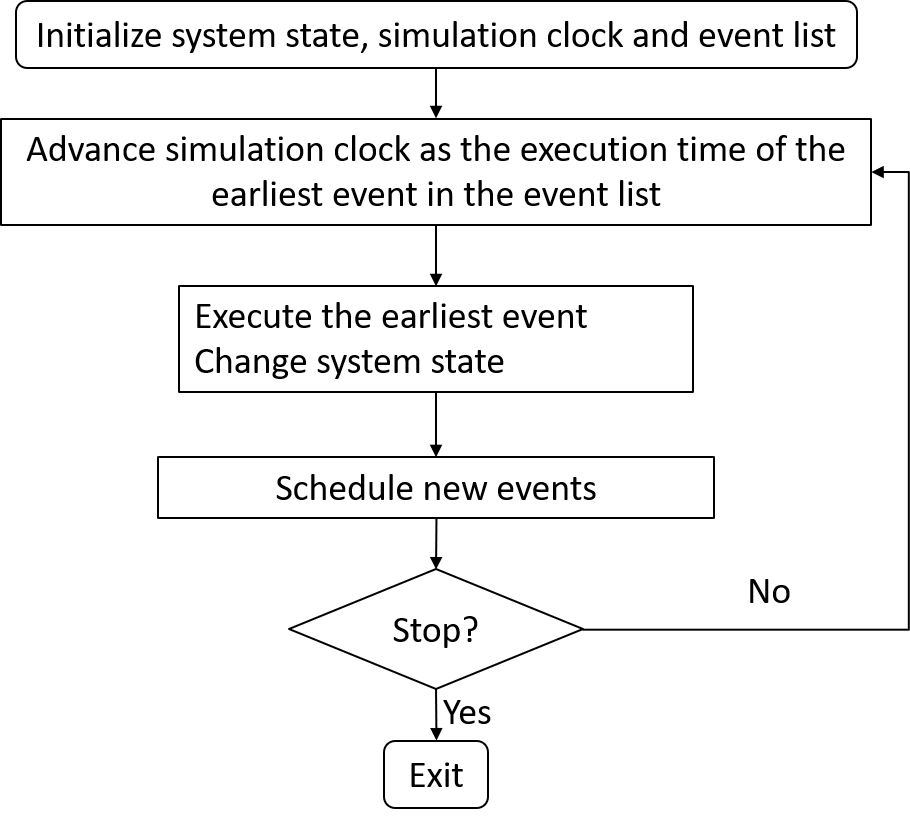
\includegraphics[width=0.6\textwidth]{Figures/EventSimAlgo.png}
	\caption{Event-based simulation algorithm.}
	\label{fig:EventSimAlgo}
\end{figure}

An equivalent mathematical programming model exists if the following assumptions are satisfied:
\begin{enumerate}
	\item State variables are integer.
	\item For all event $e^{\xi}$, the \textit{scheduling conditions} are in the form of $a^{\xi}_s\le s \le b^{\xi}_s$ combined with logic operator ``AND", where $s$ is a state variable, and $a^{\xi}_s$ and $b^{\xi}_s$ are lower and upper bounds.
	\item The scheduling conditions is independent of the history and not changed along time. (It could be possible to define more state variables in case of history dependence and time-variant scheduling conditions.)
	\item An event execution of $e^{\xi}$ leads to integer increment or decrement equal to $\Delta^{\xi}_s$ of certain state variables $s$, and $\Delta^{\xi}_s$ is not changed along time.
	\item The delay between scheduling and execution time of an event $e^{\xi}$, denoted by $t^{\xi}$, is random variate. They can be generated independently from the simulation run. (\textit{This point is different from ERG. In ERG, the delay is dependent on the edge, i.e, a couple of events, but I consider delay dependent on a single event.})
	\item For all events $e^{\xi}$, the number of executions $I^{\xi}$ is known before simulation.
\end{enumerate}

\begin{table}[h]
	\begin{tabular}{ll}
		$e^{\xi}$ & event of type $\xi$\\
		$s$& state variable\\
		$S$& set of all state variables\\
		$S^{\xi}$  & set of state variables whose value is conditioned for scheduling event $e^{\xi}$.\\
		$\Theta^{\xi+}$ & the set of state variables that event $e^{\xi}$ will increase its value.\\
		$\Theta^{\xi-}$ & the set of state variables that event $e^{\xi}$ will decrease its value.\\
		$\Theta^{\xi}$ & $\Theta^{\xi+}\cap\Theta^{\xi-}$\\
		$E^{s+}$ & set of events whose execution increases the value of state variable $s$.\\
		$E^{s-}$  & set of events whose execution decreases the value of state variable $s$.\\
		$\Delta^{\xi}_s$ & increment or decrement of state variable $s$ when event $e^{\xi}$ is executed.\\
		$I^{\xi}$ & total number of executions of event $e^{\xi}$\\
		$L^{s+}$& total number of  times that state variable $s$ is increased.\\
		$L^{s-}$ & total number of  times that state variable $s$ is decreased.\\
		$t^{\xi}$ & delay between scheduling and execution of event $e^{\xi}$.\\
		$t^{\xi}_i$ & delay between $i$-th scheduling and its execution of event $e^{\xi}$.\\
	\end{tabular}
\caption{Notations}
\end{table}


\textbf{Preparation} Event $e^{\xi}$ is expanded into a series of events $e^{\xi,0}$, $e^{\xi,1}$, ..., $e^{\xi,\Delta^{\xi}}$, where $\Delta^{\xi}$ is equal to the maximum among $\Delta^{\xi}_s$ for all $s\in \Theta^{\xi}$. The expansion is conducted as follows. First, event $e^{\xi,0}$ is executed as soon as all the scheduling conditions are satisfied, and the state variables $s\in \Theta^{\xi}$ are not changed. Then, event $e^{\xi,1}$ is executed after $t^{\xi}$ time unit after an execution of $e^{\xi,0}$. For all $s\in \Theta^{\xi}$, if $\Delta^{\xi}_s\ge \delta$,  $e^{\xi,\delta}$ will increase or decrease $s$ by one, for all $\delta=1,...,\Delta^{\xi}$. The $i$-th execution of event $e^{\xi,\delta}$ for $\delta=1,...,\Delta^{\xi}$ are simultaneous.



\begin{table}[h]
	\begin{tabular}{ll}
		$e^{\xi,\delta}_i\ge 0$ 	& time of $i$-th execution of event $e^{\xi,\delta}$\\
		$\tau^{s+}_{l}\ge 0$ 			& time when state variable $s$ is increased for the $l$-th time.  \\
		$\tau^{s-}_{l}\ge 0$ 			& time when state variable $s$ is decreased for the $l$-th time. \\
		$x^{\xi}_{i,i^{'}}\in \{0,1\}$ 	& equal to 1 if the $i^{'}$ execution of event $e^{\xi}$ is the $i$-th scheduled one. \\
		$y^{\xi,\delta,s+}_{i,l}\in \{0,1\}$ & equal to 1 if the $i$-th execution of event $e^{\xi}$ is the $l$-th time that state variable $s$ in increased.\\
		$y^{\xi,\delta,s-}_{i,l}\in \{0,1\}$ &equal to 1 if the $i$-th execution of event $e^{\xi}$ is the $l$-th time that state variable $s$ in decreased.\\
		$z^{\xi,s+}_{i,l}\in \{0,1\}$ & equal to 1 if the $i$-th scheduling of event $e^{\xi}$ is later than $\tau^{s+}_{l}$.\\
	\end{tabular}
\caption{Decision variables}
\end{table}


\textbf{Constraints (A)} The constraints below imply that event $e^{\xi,1}$ is scheduled to execute with a delay $t^{\xi}$, after an execution of $e^{\xi,0}$. 
\begin{eqnarray}
e^{\xi,1}_{i^{'}} - e^{\xi,0}_{i} \ge t^{\xi}_{i} +M(x^{\xi}_{i,i^{'}}-1) && \forall \xi, i, i ^{'}=1,...,I^{\xi}\label{eq::A1}
\end{eqnarray}

It should be noticed that, if multiple executions of the same event $e^{\xi}$ are allow to exist in the future event list simultaneously, the execution of $e^{\xi,1}$ scheduled by the $i$-th execution of $e^{\xi,0}$ may be not the $i$-th execution of $e^{\xi,1}$. Thus, binary variables $x^{\xi}_{i,i^{'}}$ are introduced, and it is equal to one if the $i^{'}$ execution of event $e^{\xi,1}$ is scheduled by the $i$-th execution of event $e^{\xi,0}$. Since each execution of $e^{\xi,0}$ can schedule one and only one execution of $e^{\xi,1}$, the following constraints should also be satisfied:
\begin{eqnarray}
\sum_{i=1}^{N^{\xi}} x^{\xi}_{i,i^{'}} = 1&& \forall\ \xi, i^{'}=1,...,I^{\xi}\\
\sum_{i^{'}=1}^{N^{\xi}} x^{\xi}_{i,i^{'}} = 1 && \forall\ \xi,i=1,...,I^{\xi}
\end{eqnarray}

If up to $\alpha^{\xi}$ multiple executions of event $e^{\xi}$ are allowed, the following constraints can be added:

\begin{eqnarray}
e^{\xi,0}_{i} - e^{\xi,1}_{i-\alpha^{\xi}} \ge 0 && \forall\ \xi,\ i=\alpha^{\xi}+1,...,I^{\xi} \\
\sum_{i^{'}=i+\alpha^{\xi}}^{I^{\xi}} x^{\xi}_{i,i^{'}}=0&& \forall\ \xi,\ i=1,...,I^{\xi}-\alpha^{\xi}\\
\sum_{i=1}^{i^{'}-\alpha^{\xi}} x^{\xi}_{i,i^{'}}=0&&\forall\ \xi,\ i^{'}=\alpha^{\xi}+1, ..., I^{\xi}
\end{eqnarray}

If $\alpha^{\xi}$ is equal to one, the constraints (A) are reduced to:
\begin{eqnarray}
e^{\xi,1}_{i} - e^{\xi,0}_{i} \ge t^{\xi}_{i} && \forall \xi, i=1,...,I^{\xi}\\
e^{\xi,0}_{i} - e^{\xi,1}_{i-1} \ge 0&& \forall\ \xi,\ i=2,...,I^{\xi} 
\end{eqnarray}

\textbf{Constraints (B)} Binding $e^{\xi,\delta}_i$ and $\tau^{s+}_l,\ \tau^{s-}_l$:
\begin{eqnarray}
\tau^{s+}_l - e^{\xi,\delta}_i \ge M(y^{\xi,\delta,s+}_{i,l}-1)&&\forall\ s\in S,e^{\xi}\in E^{s+},\delta=1,..,\Delta^{\xi}_s,i=1,..,I^{\xi},l=1,..,L^{s+} \\
e^{\xi,\delta}_i - \tau^{s+}_l \ge M(y^{\xi,\delta,s+}_{i,l}-1)&&\forall\ s\in S,e^{\xi}\in E^{s+},\delta=1,..,\Delta^{\xi}_s,i=1,..,I^{\xi},l=1,..,L^{s+}\\
\tau^{s-}_l - e^{\xi,\delta}_i \ge M(y^{\xi,\delta,s-}_{i,l}-1)&&\forall\ s\in S,e^{\xi}\in E^{s-},\delta=1,..,\Delta^{\xi}_s,i=1,..,I^{\xi},l=1,..,L^{s-}\\
e^{\xi,\delta}_i - \tau^{s-}_l \ge M(y^{\xi,\delta,s-}_{i,l}-1)&&\forall\ s\in S,e^{\xi}\in E^{s-},\delta=1,..,\Delta^{\xi}_s,i=1,..,I^{\xi},l=1,..,L^{s-}\\
\sum_{\begin{subarray}{c} \xi:e^{\xi}\in E^{s+} \\ i=1,...,I^{\xi}\\\Delta=1,..., \Delta^{\xi}_s\end{subarray}} y^{\xi,\delta,s+}_{i,l}=1&& \forall\ s\in S,l=1,...,L^{s+}\\
\sum_{l=1,...,L^{s+}} y^{\xi,\delta,s+}_{i,l}=1&&\forall\ \xi,s\in \Theta^{\xi+},i=1,...,I^{\xi},\delta=1,...,\Delta^{\xi}_{s}\\
\sum_{\begin{subarray}{c} \xi:e^{\xi}\in E^{s-} \\ i=1,...,I^{\xi}\\\Delta=1,..., \Delta^{\xi}_s\end{subarray}} y^{\xi,\delta,s-}_{i,l}=1&& \forall\ s\in S,l=1,...,L^{s-}\\
\sum_{l=1,...,L^{s-}} y^{\xi,\delta,s-}_{i,l}=1&&\forall\ \xi, s\in \Theta^{\xi-}, i=1,...,I^{\xi},\delta=1,...,\Delta^{\xi}_{s}\\
\end{eqnarray}

Binary variables $y^{\xi,\delta,s+}_{i,l}\in \{0,1\}$ are equal to one if the $i$-th execution of event $e^{\xi,\delta}$ is the $l$-th time that state variable $s$ in increased. Since events $e^{\xi,1},...,e^{\xi,\Delta^{\xi}_s}$ are expanded from one event $e^{\xi}$, and they are executed simultaneously, the following constraints are also added:
\begin{eqnarray}
e^{\xi,\delta}_i = e^{\xi,1}_i && \forall\ \xi,\ i=1,...,I^{\xi}, \delta=1,...,\Delta^{\xi}\\
y^{\xi,\delta,s+}_{i,l+\delta-1} = y^{\xi,1,s+}_{i,l} &&\forall\ \xi,\ s\in\Theta^{\xi+},\ \delta=1,...,\Delta^{\xi}_s,\ i=1,...,I^{\xi}, \ l=1,...,L^{s+}-\Delta^{\xi}_s+1\\
y^{\xi,\delta,s-}_{i,l+\delta-1} = y^{\xi,1,s-}_{i,l} &&\forall\ \xi,\ s\in\Theta^{\xi-},\ \delta=1,...,\Delta^{\xi}_s,\ i=1,...,I^{\xi}, \ l=1,...,L^{s-}-\Delta^{\xi}_s+1
\end{eqnarray}


\textbf{Constraints (C)} To trigger event $e^{\xi,0}$, the conditions $a^{\xi}_s\le s\le b^{\xi}_s$ for all state variable $s\in S^{\xi}$ should be satisfied. $s\in S^{\xi}$ can be categorized into one of the following three situations:
\begin{itemize}
	\item event $e^{\xi}$ does not change the value of $s$, i.e., $s\notin \Theta^{\xi}$.
	\item event $e^{\xi}$ increases the value of $s$, i.e., $s\in \Theta^{\xi+}$. 
	\item event $e^{\xi}$ decreases the value of $s$, i.e., $s\in \Theta^{\xi-}$. 
\end{itemize}

If event $e^{\xi}$ does not change the value of $s$, or if it is executed after being scheduled with positive delay, i.e., $s\notin \Theta^{\xi}$ or $t^{\xi}>0$, the following constraints are applied:
\begin{eqnarray}
e^{\xi,0}_{i} - \tau_{l}^{s+} \le Mz^{\xi,s+}_{i,l} & \forall\ \xi,i=1,...,I^{\xi},\ s\in S^{\xi}, l=1,....,L^{s+}\\
e^{\xi,0}_{i} - \tau_{l}^{s-} \le Mz^{\xi,s-}_{i,l} & \forall\ \xi,\ i=1,...,I^{\xi},\ s\in S^{\xi}, l=1,....,L^{s-}\\
e^{\xi,0}_{i} - \tau_{l}^{s-} \ge -M\hat{z}^{\xi,s-}_{i,l}& \forall\ \xi,\ i=1,...,I^{\xi},\ s\in S^{\xi}, l=1,....,L^{s-}\\
e^{\xi,0}_{i} - \tau_{l}^{s+} \ge -M\hat{z}^{\xi,s+}_{i,l}& \forall\ \xi,\ i=1,...,I^{\xi},\ s\in S^{\xi}, l=1,....,L^{s+}\\
%e^{\xi,0}_{i} - \tau_{s_0+l-b^{\xi}_{s}}^{s-} \ge -M\hat{z}^{\xi,s-}_{i,l}& \forall\ \xi,\ i=1,...,I^{\xi},\ s\in S^{\xi}, l=1,....,L^{s-}??\\
%e^{\xi,0}_{i} - \tau_{-s_0+l+a^{\xi}_{s}}^{s+} \ge -M\hat{z}^{\xi,s+}_{i,l}& \forall\ \xi,\ i=1,...,I^{\xi},\ s\in S^{\xi}, l=1,....,L^{s+}??\\
z^{\xi,s+}_{i,l}+\hat{z}^{\xi,s-}_{i,s_0+l-b^{\xi}_{s}}\le 1&??\\
z^{\xi,s-}_{i,l}+\hat{z}^{\xi,s+}_{i,-s_0+l+a^{\xi}_{s}}\le 1&??\\
%z^{\xi,s+}_{i,l}+\hat{z}^{\xi,s-}_{i,l}\le 1&??\\
%z^{\xi,s-}_{i,l}+\hat{z}^{\xi,s+}_{i,l}\le 1&??
\end{eqnarray}

\begin{eqnarray}
e^{\xi,0}_{i} - \tau_{l}^{s+} \ge M(z^{\xi,s+}_{i,l}-1) & \forall\ \xi,i=1,...,I^{\xi},\ s\in S^{\xi}, l=1,....,L^{s+}\\
\tau_{l}^{s+} - e^{\xi,0}_{i} > -Mz^{\xi,s+}_{i,l}& \forall\ \xi,\ i=1,...,I^{\xi},\ s\in S^{\xi}, l=1,....,L^{s+}\\
e^{\xi,0}_{i} - \tau_{l}^{s-} \ge M(z^{\xi,s-}_{i,l}-1) & \forall\ \xi,\ i=1,...,I^{\xi},\ s\in S^{\xi}, l=1,....,L^{s-}\\
\tau_{l}^{s-} - e^{\xi,0}_{i} > -Mz^{\xi,s-}_{i,l}& \forall\ \xi,\ i=1,...,I^{\xi},\ s\in S^{\xi}, l=1,....,L^{s-}\\
\end{eqnarray}







If $e^{\xi,0}_{i}$ is executed after $\tau_{l}^{s+}$($\tau_{l}^{s-}$), $z^{\xi,s+}_{i,l}$($z^{\xi,s-}_{i,l}$) is equal to one. If $e^{\xi,0}_{i}$ is executed before $\tau_{l}^{s+}$($\tau_{l}^{s-}$), $\hat{z}^{\xi,s+}_{i,l}$($\hat{z}^{\xi,s-}_{i,l}$) is equal to one.


If event $e^{\xi}$ increases the value of $s$, and it is executed immediately when scheduled, i.e., $s\in \Theta^{\xi+}$ and $t^{\xi}=0$, the following constraint should be applied:
\begin{eqnarray}
e^{\xi,0} - \tau^{s-}_{s_0+l-1-b} \ge M(y^{\xi,1,s+}_{i,l}-1)\\
e^{\xi,0} - \tau^{s-}_{s_0+l-1-a} \le M(1-y^{\xi,1,s+}_{i,l})
\end{eqnarray}

If event $e^{\xi}$ decreases the value of $s$, and it is executed immediately when scheduled, i.e., $s\in \Theta^{\xi-}$ and $t^{\xi}=0$, the following constraint should be applied:
\begin{eqnarray}
e^{\xi,0} - \tau^{s+}_{-s_0+l-1+a} \ge M(y^{\xi,1,s-}_{i,l}-1)\\
e^{\xi,0} - \tau^{s+}_{-s_0+l-1+b} \le M(1-y^{\xi,1,s-}_{i,l})
\end{eqnarray}



\newpage
\subsection{Mathematical programming representation of simulation model - V3}
Event-scheduling algorithm for DES. 

\begin{figure}[h]
	\centering
	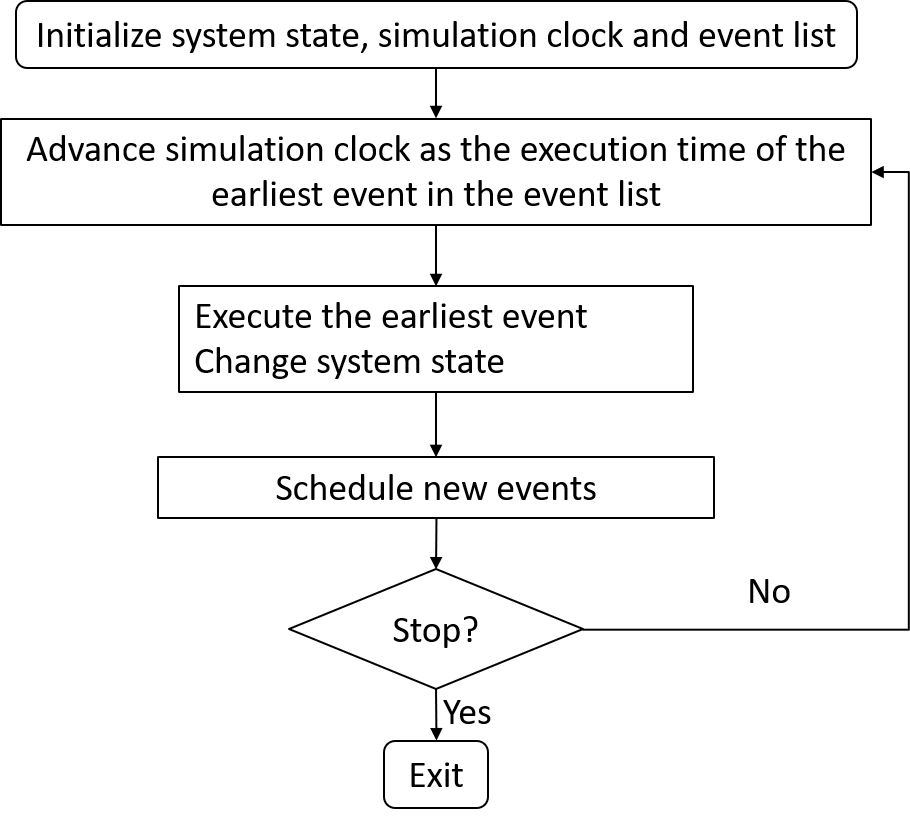
\includegraphics[width=0.8\textwidth]{Figures/EventSimAlgo.png}
	\caption{Event-based simulation algorithm.}
\end{figure}


An equivalent mathematical programming model exists if the following assumptions are satisfied:
\begin{enumerate}
	% \item State variables are integer.
	\item For all event $e^{\xi}$, the \textit{scheduling conditions} are in the form of $a^{\xi}_s\le s \le b^{\xi}_s$ combined with logic operator ``AND", where $s$ is a state variable, and $a^{\xi}_s$ and $b^{\xi}_s$ are lower and upper bounds.
	\item The scheduling conditions is independent of the history and not changed along time. (It could be possible to define more state variables in case of history dependence and time-variant scheduling conditions.)
	\item An event execution of $e^{\xi}$ leads to (integer) increment or decrement equal to $\Delta^{\xi}_s$ of certain state variables $s$, and $\Delta^{\xi}_s$ is not changed along time. (A direct evaluation can be modeled in this way.)
	\item The delay between scheduling and execution time of an event $e^{\xi}$, denoted by $t^{\xi}$, is random variate. They can be generated independently from the simulation run. (\textit{This point is different from ERG. In ERG, the delay is dependent on the edge, i.e, a couple of events, but I consider delay dependent on a single event.})
	\item For all events $e^{\xi}$, the number of executions $N^{\xi}$ is known before simulation.
\end{enumerate}

\begin{table}[h]
	\begin{tabular}{lll}
		$e^{\xi,0}_{i}\ge 0$ & $i$=1,...,$I^{\xi}$& the $i$-th scheduling time of event $e^{\xi}$.\\
		$e^{\xi,1}_{i}\ge 0$ & $i$=1,...,$I^{\xi}$& the $i$-th execution time of event $e^{\xi}$.\\
		$\mathcal{E}_k\ge 0$ &$k$=0,...,$K$& time of the $k$-th execution of any events.\\
		$u^s_k\in \mathbb{Z}$ &$k$=0,...,$K$& value of state variable $s$ just after the $k$-th event.\\
		$w^{\xi}_{i,k}\in \{0,1\}$ &$k$=1,...,$K$& binding $e^{\xi,1}_i$ and $\mathcal{E}_k$.\\
		$x^{\xi}_{i,k}\in\{0,1\}$ &$k$=0,...,$K$& equal to one if $\mathcal{E}_k$ schedules $e^{\xi,0}$.\\
		$y^{\xi}_{i,i^{'}}\in\{0,1\}$&& binding $e^{\xi,0}_i$ and $e^{\xi,1}_{i^{'}}$ in case of overtaking.\\
		$z^{\xi}_{k}\in\{0,1\}$ &$k$=0,...,$K$& equal to one if the condition for scheduling $e^{\xi}$ is true right after $\mathcal{E}_k$.\\ 
		$v^{\xi,s,0}_k\in\{0,1\}$ &$k$=0,...,$K$& equal to one if $s_k\le a^{\xi,s}-1$\\
		$v^{\xi,s,1}_k\in\{0,1\}$ &$k$=0,...,$K$& equal to one if $s_k\ge b^{\xi,s}-1$\\
		$r^{\xi}_k\in \mathbb{Z}$ &$k$=0,...,$K$& number of existing parallel executions of $e^{\xi,1}_i$ after $\mathcal{E}_k$ before scheduling.\\
		$n^{\xi}_k\in \mathbb{Z}$ & $k$=0,...,$K$ & number of scheduled executions of $e^{\xi,1}_i$ after $\mathcal{E}_k$ before scheduling.\\
	\end{tabular}
\caption{Notation}
\end{table}

\textbf{Constraints (A):} binding $e^{\xi,1}_i$ and $\mathcal{E}_k$:
\begin{eqnarray}
	e^{\xi,1}_i-\mathcal{E}_k\ge M(w^{\xi}_{i,k}-1) &A1& \forall\ \xi,i,k\\
	\mathcal{E}_k-e^{\xi,1}_i\ge M(w^{\xi}_{i,k}-1) &A2& \forall\ \xi,i,k\\
	\sum_{k} w^{\xi}_{i,k} =1&A3& \forall\ \xi,i\\
	\sum_{\xi,i} w^{\xi}_{i,k} =1&A4& \forall\ k\\
	\sum_{k} kw^{\xi}_{i+1,k} - \sum_{k} kw^{\xi}_{i,k} \ge 1&A5& \forall\ \xi,i
\end{eqnarray}

\textbf{Constraints (B):} binding $e^{\xi,0}_i$ and $e^{\xi,1}_{i^{'}}$, where $\alpha^{\xi}$ is the maximal number of executions existing simultaneously in the event list:
\begin{eqnarray}
e^{\xi,1}_{i^{'}} - e^{\xi,0}_{i} \ge t^{\xi}_{i} +M(y^{\xi}_{i,i^{'}}-1) &B1& \forall \xi, i, i ^{'}=1,...,N^{\xi}\\
e^{\xi,0}_{i} - e^{\xi,1}_{i^{'}}  \ge -t^{\xi}_{i} +M(y^{\xi}_{i,i^{'}}-1) &B2& \forall \xi, i, i ^{'}=1,...,N^{\xi}\\
\sum_{i=1}^{N^{\xi}} y^{\xi}_{i,i^{'}} = 1&B3& \forall\ \xi, i^{'}=1,...,N^{\xi}\\
\sum_{i^{'}=1}^{N^{\xi}} y^{\xi}_{i,i^{'}} = 1 &B4& \forall\ \xi,i=1,...,N^{\xi}\\
%e^{\xi,0}_{i} - e^{\xi,1}_{i-\alpha^{\xi}} \ge 0 && \forall\ \xi,\ i=\alpha^{\xi}+1,...,N^{\xi} \\
\sum_{i^{'}=i+\alpha^{\xi}}^{N^{\xi}} y^{\xi}_{i,i^{'}}=0&B5& \forall\ \xi,\ i=1,...,N^{\xi}-\alpha^{\xi}\\
\sum_{i=1}^{i^{'}-\alpha^{\xi}} y^{\xi}_{i,i^{'}}=0&B6&\forall\ \xi,\ i^{'}=\alpha^{\xi}+1, ..., N^{\xi}
\end{eqnarray}
If $\alpha^{\xi}=1$, variables $y^{\xi}_{i,i^{'}}$ are redundant and constraints (B) are reduced to:
\begin{eqnarray}
e^{\xi,1}_{i} - e^{\xi,0}_{i} = t^{\xi}_{i} &B1& \forall \xi, i=1,...,N^{\xi}
% e^{\xi,0}_{i} - e^{\xi,1}_{i-1} \ge 0 && \forall\ \xi,\ i=2,...,N^{\xi} 
\end{eqnarray}
Number of executions of event $e^{\xi}$ waiting in the event list can be a state variable $n^{\xi}$, and one condition for scheduling an $e^{\xi}$ is $n^{\xi}\le \alpha^{\xi}$. Thus, it can be managed as a generic scheduling condition.

\textbf{Constraints (C):} event $e^{\xi}$ can be scheduled right after $\mathcal{E}_k$ if all state variables $s$ satisfies condition $a^{\xi}_{s}\le s_k\le b^{\xi}_{s}$. 
\begin{eqnarray}
e^{\xi,0}_i-\mathcal{E}_{k} \ge M(x^{\xi}_{i,k}-1)&C1& \forall\ \xi,k,i\\
\mathcal{E}_{k} -e^{\xi,0}_i\ge M(x^{\xi}_{i,k}-1)&C2& \forall\ \xi,k,i\\
\sum_{k} x^{\xi}_{i,k} =1&C3& \forall\ \xi,i\\
b^{\xi,s} - u^s_k \ge M(z^{\xi}_{k}-1)&C4& \forall\ \xi, k,s\\
% - u^s_k \ge U^{s}(z^{\xi}_{k}-1)-b^{\xi,s}z^{\xi}_{k}&C4& \forall\ \xi, k,s\\
 u^s_k - a^{\xi,s} \ge M(z^{\xi}_{k}-1)&C5& \forall\ \xi, k,s\\
%u^s_k  \ge a^{\xi,s}z^{\xi}_{k} -L^{s}(z^{\xi}_{k}-1)&C5& \forall\ \xi, k,s\\
u^s_k -  (b^{\xi,s}+1) \ge M(v^{\xi,s,1}_k-1) &C6& \forall\ \xi,k,s\\
%u^s_k \ge (b^{\xi,s}+1)v^{\xi,s,1}_k -L^s(v^{\xi,s,1}_k-1)&C6& \forall\ \xi,k,s\\
( a^{\xi,s}-1) - u^s_k \ge M(v^{\xi,s,0}_k-1) &C7& \forall\ \xi,k,s\\
% - u^s_k \ge U^s(v^{\xi,s,0}_k-1)-(a^{\xi,s}-1)v^{\xi,s,0}_k &C7& \forall\ \xi,k,s\\
1 - z^{\xi}_{k} \le \sum_{s\in S^{\xi}} v^{\xi,s,0}_k + \sum_{s\in S^{\xi}} v^{\xi,s,1}_k + v^{\xi,r}_k + v^{\xi,N}_k&C8&\forall\ \xi,k\\
\sum_{i=1}^{N^{\xi}}x^{\xi}_{i,k} = z^{\xi}_k&C9&\forall\ \xi,k\\
%X^{\xi}_k  = z^{\xi}_{k}  &C90& \forall\ \xi, k\\
% - r^{\xi}_{k} \le N^{\xi} - n^{\xi}_{k} -R^{\xi}\beta^{\xi}_k&C91&\forall\ \xi, k\\
%N^{\xi} - n^{\xi}_{k} \le R^{\xi} - r^{\xi}_{k} +N^{\xi}\beta^{\xi}_k&C92&\forall\ \xi, k\\
%X^{\xi}_k\ge R^{\xi}(z^{\xi}_k + \beta^{\xi}_k-1) - r^{\xi}_{k}&C93&\forall\ \xi, k\\
%X^{\xi}_k\ge N^{\xi}z^{\xi}_k - N^{\xi}\beta^{\xi}_k - n^{\xi}_{k}&C94&\forall\ \xi, k\\
\sum_{k} kx^{\xi}_{i+1,k} - \sum_{k} kx^{\xi}_{i,k} \ge 1&C10& \forall\ \xi,i
\end{eqnarray}

%If $r^{\xi}_{max}=1$, then constraints C9 to C94 is reduced to 
%\begin{eqnarray}
%\sum_{i=1}^{N^{\xi}}x^{\xi}_{i,k} = z^{\xi}_k&C9&\forall\ \xi,k
%\end{eqnarray}

\textbf{Constraints (D):} evolution of state variables
\begin{eqnarray}
u^{s}_{k} = u^s_{k-1} + \sum_{\xi} \sum_{i=1}^{N^{\xi}} w^{\xi}_{i,k} \Delta^{\xi,s}&D1& \forall\ s,k\\
r^{\xi}_k = r^{\xi}_{k-1} + X^{\xi}_{k-1} - \sum_i w^{\xi}_{i,k} &D2& \forall\ \xi,k\\
R^{\xi} - r^{\xi}_k \ge z^{\xi}_k&D3& \forall\ \xi,k\\
r^{\xi}_k  \ge R^{\xi}v^{\xi,r}_k&D4& \forall\ \xi,k\\
n^{\xi}_k = n^{\xi}_{k-1} + X^{\xi}_{k-1} &D5& \forall\ \xi,k\\
N^{\xi} - n^{\xi}_k \ge z^{\xi}_k&D6&\forall\ \xi,k\\
n^{\xi}_k \ge N^{\xi}v^{\xi,N}_k&D7&\forall\ \xi,k
\end{eqnarray}

\textbf{Constraints (E):} others
\begin{eqnarray}
\mathcal{E}_{0} = 0&E1&\\
\mathcal{E}_{k}-\mathcal{E}_{k-1}\ge 0&E1&\forall\ k
\end{eqnarray}

%Constraints (D): for zero-delay event $e^{\xi}$, $\alpha^{\xi}$ is equal to 1. Thus, $e^{\xi,0}_{i+1}$ can be scheduled after the execution of $e^{\xi,1}_{i}$
%\begin{eqnarray}
%x^{\xi}_{i+1,k}\le \sum_{k^{'}=1}^{k} w^{\xi}_{i,k^{'}} && \forall\ \text{zero-delay event}\ e^{\xi}
%\end{eqnarray}

\textbf{Objective function:} with the constraints above, there is a unique solution in terms of event occurring times (solution of the binary variables could be multiple in case of multiple simultaneous events). Thus, the objective can be any function of event occurring time. I tried minimize/maximize the sum of $\mathcal{E}_k$, and they give the same solution.

\textbf{Conditions for a variable $x$ to be \textit{resource-type} are not valid any more.}
\begin{enumerate}
\item $\forall\ \xi$ and $s$, upper bound $b^{\xi}_s$ is monotonically increasing on $x$.
\item  $\forall\ \xi$ and $s$, lower bound $a^{\xi}_s$ is monotonically decreasing on $x$.
%\item $\forall\ \xi$, maximal number of executions waiting in the event list simultaneously $\alpha^{\xi}$ in monotonically increasing on $x$.
\end{enumerate}

The reason is that increasing $b^{\xi}_s$ or decreasing $a^{\xi}_s$ will tighten constraints C6 and C7. To be simple, we consider $b$ only. 
\begin{eqnarray}
b - u^s_k \ge M(z^{\xi}_{k}-1)&C4-b& \forall\ \xi, k,s\\
u^s_k -  (b+1) \ge M(v^{\xi,s,1}_k-1) &C6-b& \forall\ \xi,k,s
\end{eqnarray}
(when $u=b+1$, event $e^{\xi}$ cannot be scheduled.)

If $b$ is increased to $b+1$:
\begin{eqnarray}
(b+1) - u^s_k \ge M(z^{\xi}_{k}-1)&C4-(b+1)& \forall\ \xi, k,s\\
u^s_k -  (b+2) \ge M(v^{\xi,s,1}_k-1) &C6-(b+1)& \forall\ \xi,k,s
\end{eqnarray}
(when $u=b+1$, event $e^{\xi}$ must be scheduled.)

A group of relaxed constraints are:
\begin{eqnarray}
(b+1) - u^s_k \ge M(z^{\xi}_{k}-1)&C4-(b+1)& \forall\ \xi, k,s\\
u^s_k -  (b+1) \ge M(v^{\xi,s,1}_k-1) &C6-(b)& \forall\ \xi,k,s
\end{eqnarray}
(when $u=b+1$, event $e^{\xi}$ can be scheduled or not.)


Todo: 
\begin{enumerate}
	\item What kind of performance indicators can be used? (Regular function of time, in scheduling area. Weighted sum, maximum. Refer to book on scheduling.)
\end{enumerate}

\newpage

\subsection{Merge}
\begin{figure}[h]
	\centering
	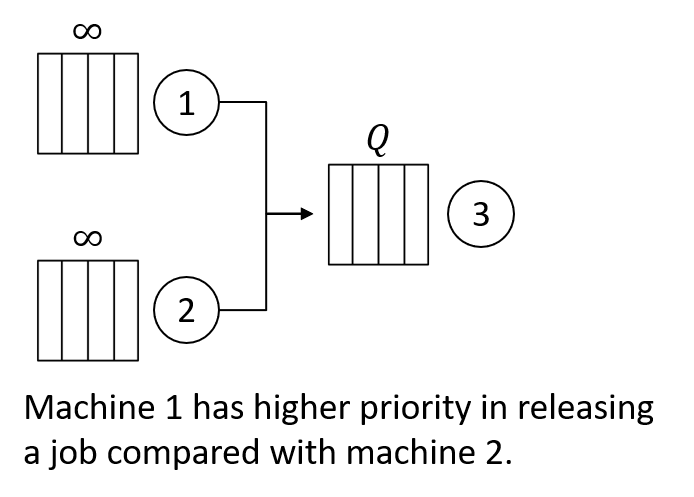
\includegraphics[width=0.9\textwidth]{Figures/merge.png}
	\caption{Example: merge.}
\end{figure}

\begin{table}[h]
	\begin{tabular}{|llllll|}\hline
		Variable&Event & Condition to schedule & Delay&\# executions& State change\\\hline
		$e^{s,1}$&Start m1 	& $m^1\le 0$ & $0$&1& $m^1++$ \\\hline
		$e^{f,1}$&Finish m1 & $1\le m^1\le 1$ 	& $t^1$ &1& $m^1++$\\\hline
		$e^{d,1}$&Depart m1& $m^1\ge2\ AND$&$0$ &1 & $m^1 = m^1-2,\ q--$\\
											&&$ q\ge 1$ &&&\\\hline
		$e^{s,2}$&Start m2 	& $m^2\le 0$ & $0$ &1& $m^2++$ \\	\hline
		$e^{f,2}$&Finish m2 & $1\le m^2\le 1$ 	& $t^2$ &1 & $m^2++$\\\hline
		$e^{d,2}$&Depart m2& $m^2\ge2\ AND$&$0$  &1& $m^2=m^2-2,\ q--$\\
						&&$\ q\ge 1\ AND$&&&\\
						&&$\ m^1\le 1 $ & &&\\\hline
		$e^{s,3}$& Start m3 & $m^3 \le 0\ AND$&$0$  &1& $m^3++,\ q++$\\
						&&$\ q\le Q-1$ & &&\\\hline
		$e^{d,3}$& Depart m3 & $m^3 \ge 1$ & $t^3$  &1& $m^3--$\\\hline
	\end{tabular}
	\caption{Merge-S3M111}
\end{table}

MP model:
\begin{eqnarray}
\min{\sum_{k}\mathcal{E}_k}\\
e^{(\xi,j),1}_i - \mathcal{E}_{k}\ge M(w^{\xi,j}_{i,k}-1)&&\xi\in\{s,f,d\}, j\in\{1,2,3\},\forall i,k \\
\mathcal{E}_{k} - e^{(\xi,j),1}_i\ge M(w^{\xi,j}_{i,k}-1)&&\xi\in\{s,f,d\}, j\in\{1,2,3\},\forall i,k \\
\sum_{k} w^{\xi,j}_{i,k} =1&& \forall\ \xi\in\{s,f,d\}, j\in\{1,2,3\},i\\
\sum_{(\xi,j),i} w^{\xi,j}_{i,k} =1&& \forall\ k\\
\sum_{k} kw^{\xi,j}_{i+1,k} - \sum_{k} kw^{\xi,j}_{i,k} \ge 1&& \forall\  \xi\in\{s,f,d\}, j\in\{1,2,3\},i\\
e^{s,j,1}_{i} - e^{s,j,0}_{i} \ge 0 && j =1,2,3, \forall \ i\\
e^{f,j,1}_{i} - e^{f,j,0}_{i} \ge t^j_{i}&& j =1,2, \forall \ i\\
e^{d,j,1}_{i} - e^{d,j,0}_{i} \ge 0 && j =1,2, \forall \ i\\
e^{d,3,1}_{i} - e^{d,3,0}_{i} \ge t^3_{i}&&\forall \ i \\
e^{\xi,j,0}_i-\mathcal{E}_{k} \ge M(x^{\xi,j}_{i,k}-1)&& \forall\ \xi\in\{s,f,d\},j=1,2,3,k,i\\
\mathcal{E}_{k} -e^{\xi,j,0}_i\ge M(x^{\xi,j}_{i,k}-1)&& \forall\ \xi\in\{s,f,d\},j=1,2,3,k,i\\
m^j_k=m^j_{k-1} + \sum_{i=1}^{N^{j}} (w^{s,j}_{i,k}  + w^{f,j}_{i,k} - 2w^{d,j}_{i,k})&& j=1,2, \forall\ k\\
m^3_k=m^3_{k-1} + \sum_{i=1}^{N^{3}} (w^{s,3}_{i,k} - w^{d,3}_{i,k})&&\forall\ k\\
q_k = q_{k-1} + \sum_{i=1}^{N^{3}} w^{s,3}_{i,k} - \sum_{i=1}^{N^{1}} w^{d,1}_{i,k} - \sum_{i=1}^{N^{2}} w^{d,2}_{i,k}\\
m^j_k \ge M(z^{s,j}_{k}-1)&& j=1,2,3, \forall \ k\\
1- m^j_k \ge M(z^{f,j}_{k}-1)&& j=1,2, \forall \ k\\
m^j_k - 1 \ge M(z^{f,j}_{k}-1)&& j=1,2, \forall \ k\\
m^j_k - 2 \ge M(z^{d,j}_{k}-1)&& j=1,2, \forall \ k\\
q_k - 1 \ge M(z^{d,j}_{k}-1)&&  j=1,2, \forall \ k\\
1 - m^1_k \ge M(z^{d,2}_{k}-1)&& \forall\ k\\
m^3_k - 1 \ge M(z^{d,3}_{k}-1)&& \forall \ k\\
(Q-1) - q_k \ge M(z^{s,3}_{k}-1)&& \forall\ k\\
\sum_{k} x^{\xi,j}_{i,k} =1&& \forall\ \xi\in\{s,f,d\}, j=1,2,3, \forall\ i,k\\
\sum_{i=1}^{N^{j}}x^{\xi,j}_{i,k} \le z^{\xi,j}_{k}&& \forall\ \xi\in\{s,f,d\}, j=1,2,3, k\\
\sum_{k} kx^{\xi,j}_{i+1,k} - \sum_{k} kx^{\xi,j}_{i,k} \ge 0 && \forall\ \xi\in\{s,f,d\}, j=1,2,3, i
\end{eqnarray}

\newpage
\subsection{Merge - 2 machines in station 3}
\begin{table}[h]
	\begin{tabular}{|llll|}\hline
		Variable&Value & Initialization& Description\\\hline
		$e^1$& 0,1,2&  2 &number of empty machines in station 1 \\\hline
		$f^1$&0,1,2	& 0 & number of finished jobs in station 1\\\hline
		$e^2$&0,1&1&number of empty machines in station 2 \\\hline
		$f^2$&0,1&0&number of finished jobs in station 2 \\\hline
		$e^3$&0,1&1&number of empty machines in station 3  \\	\hline
		$q$& 0,...,Q&Q&  number of available spaces in queue\\\hline
	\end{tabular}
	\caption{State variables: Merge-S3M211}
\end{table}


\begin{table}[h]
	\begin{tabular}{|llllll|}\hline
		Variable&Event & Condition to schedule & Delay&\# executions& State change\\\hline
	ai 	$e^{f,1}$&Finish m1 &  $1 \le  e^1 \le 2$	& $t^1$ &2& $f^1++$\\\hline
		$e^{d,1}$&Depart m1& $1\le   f^1  \le 2\ AND$&$0$ &1 & $e^1++,\ f^1--,\ q--$\\
											&&$ 1\le q\le Q$ &&&\\\hline
		$e^{s,2}$&Start m2 	& $1\le e^2\le 1$ & $0$ &1& $e^2--$ \\	\hline
		$e^{f,2}$&Finish m2 & $1\le e^2\le 1$ 	& $t^2$ &1 & $f^2++$\\\hline
		$e^{d,2}$&Depart m2&$1\le f^2 \le 1\ AND$&$0$  &1& $f^2--,e^2++,\ q--$\\
		&&$\ 1\le q\le Q\ AND$&&&\\
		&&$\ 0\le f^1\le 0 $ & &&\\\hline
		$e^{s,3}$& Start m3 & $1\le e^3\le 1\ AND$&$0$  &1& $e^3--,\ q++$\\
		&&$\ 0\le q\le Q-1$ & &&\\\hline
		$e^{d,3}$& Depart m3 & $1 \le e^3\le 1\ AND $ & $t^3$  &1& $e^3++$\\\hline
		&&$\ 0\le q\le Q-1$ & &&\\\hline
	\end{tabular}
	\caption{Events: Merge-S3M211}
\end{table}



\newpage
\subsection{Failure}



\newpage
\subsection{Jobshop}


\subsection{Identifying Resource-type variables}


\section{Gradient-based approximate cut}
\subsection{Gradient estimation}
\subsection{Gradient-based feasibility cut}


\section{Combinatorial cut generation}
\subsection{Combinatorial cut}
\subsection{Heuristic for tightening Exact combinatorial cut}

\section{Feasibility-cut-based algorithm}
The complete algorithm for solving RAP--PC is summarized in Algorithm 1. The resource capacities are initialized to the lower bound. The searching region of RAP--PC--MIP is initialized to $\Bbb{X}$, and the lower and upper bounds of the objective function, $C^L$ and $C^U$, respectively,  are set considering the upper bound and lower bound of the capacity of each resource. Lines 7 to 11 show that approximate cuts are generated and used in the model when infeasible solutions are found. Once a feasible solution is found, the upper bound $C^U$, which is also the incumbent solution, can be updated after comparing the value of the found feasible solution and that of the current incumbent. Then, all the currently used approximate cuts are replaced by exact cuts of the DIS. If there are only exact cuts in RAP--PC--MIP, the solution is the new lower bound $C^L$. The algorithm terminates when the gap between the upper bound and lower bound is within a tolerance or the time limit is exceeded.

\begin{algorithm}[h]
	\label{algo:}
	\caption{MIP--based algorithm.}
	\begin{algorithmic}[1]
		\REQUIRE ~~\\
		Lower bound $\mathbf{a}=[a_1,...,a_J]$ and upper bound $\mathbf{b}=[b_1,...,b_J]$ of resource capacity $\mathbf{x}$, such that $a_j\le x_j\le b_j\ \forall\ j=1,...,J$. \\
		Tolerance of optimality gap $\varepsilon_{opt}$.\\
		Optional input: time limit of the algorithm $T_{lim}$.\\
		\ENSURE ~~\\
		Sample-path global optimal $\mathbf{x}^*$.\\
		\STATE Initialize system with lower bound $\mathbf{x}\leftarrow\mathbf{a}$
		\STATE Initialize incumbent with upper bound $\mathbf{x}^*\leftarrow\mathbf{b}$. 
		\STATE Initialize lower bound of the objective $C^{L}\leftarrow\mathbf{c}^T\mathbf{a}$.
		\STATE Initialize upper bound of the objective $C^{U}\leftarrow\mathbf{c}^T\mathbf{b}$.
		\STATE Add initial constraints which defines $\Bbb{X}$ to the RAP--PC--MIP.
		\WHILE {$C^{U}-C^{L}>\varepsilon_{opt}$ and $T_{lim}$ is not exceeded.}
		\WHILE {There exists at least one violated performance constraint}
		\STATE Generate one approximate cut $CA(\bar{\mathbf{x}},l)$ for each violated constraints $l$ and add all the generated cuts to the RAP--PC--MIP.
		\STATE $\bar{\mathbf{x}}\leftarrow$ solution of the RAP--PC--MIP.
		\STATE Simulate the system of $\bar{\mathbf{x}}$.
		\ENDWHILE
		\STATE Update upper bound and incumbent $C^{U}\leftarrow\mathbf{c}^T\bar{\mathbf{x}},\ \mathbf{x}^*\leftarrow \bar{\mathbf{x}}$ if $\mathbf{c}^T\bar{\mathbf{x}}< C^{U}$.
		\IF {There exist approximate cuts in RAP--PC--MIP}
		\STATE For all the currently used approximate cuts $CA(\bar{\mathbf{x}}^r,l)$, find dominating infeasible solution $\bar{\mathbf{x}}_d(\bar{\mathbf{x}}^r)$ and replace approximate cuts $CA(\bar{\mathbf{x}}^r,l)$ by exact cuts $CE(\bar{\mathbf{x}}_d(\bar{\mathbf{x}}^r),l)$ of the DIS.
		\STATE $\bar{\mathbf{x}}\leftarrow$ solution of the RAP--PC--MIP.
		\STATE Simulate the system of $\bar{\mathbf{x}}$.
		\STATE Update lower bound $C^L\leftarrow \max\{\mathbf{c}^T\bar{\mathbf{x}},\ C^L\}$.
		\ENDIF	
		\ENDWHILE
	\end{algorithmic}
\end{algorithm}


\section{Numerical analysis}

\section{Conclusion}




%Reference
\bibliographystyle{apacite}
\bibliography{RAP}

\end{document}
